% cap_metodologia.tex
\chapter{Materiais e Métodos}
\label{chap:materiais_metodos}

Este capítulo descreve os dados, os modelos e o procedimento de avaliação. O procedimento foi definido para que todos os modelos recebam os mesmos dados, o mesmo tratamento e o mesmo treinamento, de modo que as diferenças observadas possam ser atribuídas aos modelos. Ele também preserva a ordem cronológica dos dados, para evitar que informação do futuro influencie o treinamento ou a avaliação.

\section{Dados}
\label{sec:dados}

O estudo utiliza medições horárias da estação Sapo, localizada em Conceição do Mato Dentro (CMD), Minas Gerais, que fazem parte do monitoramento contínuo da qualidade do ar disponibilizado pela Fundação Estadual do Meio Ambiente de Minas Gerais (FEAM) \cite{feam2026dadosmonitoramento}. A grandeza a ser prevista é a concentração de PM2,5. O principal poluente auxiliar é o PM10, o material particulado com diâmetro aerodinâmico de até 10 micrômetros. As colunas de gases e de variáveis meteorológicas do arquivo da estação (monóxido de carbono, ozônio, óxidos de nitrogênio e de enxofre, temperatura, umidade, vento, precipitação, radiação, pressão e compostos orgânicos) estão inteiramente vazias para a estação Sapo: nenhuma delas contém uma única medição. A única outra coluna com cobertura relevante é a de partículas totais em suspensão (86\% de cobertura), que não foi incluída, pois seu uso seria uma nova hipótese, e não parte da comparação.

O arquivo cobre de 1º de janeiro de 2017 a 31 de dezembro de 2023. O conjunto usado nos resultados contém 61.271 registros horários, de 4 de janeiro de 2017 a 31 de dezembro de 2023; os três primeiros dias foram descartados porque as variáveis defasadas em 24 horas e a janela de entrada de 48 horas exigem histórico anterior. Os primeiros 34.992 registros (até 31 de dezembro de 2020) foram usados em etapas exploratórias anteriores a este estudo, que orientaram algumas escolhas de projeto; os anos de 2021 a 2023 não foram usados em nenhuma etapa do desenvolvimento e formam o período de confirmação (\textit{holdout}), descrito na Seção~\ref{sec:divisao_temporal}.

\subsection{Escolha da Estação}
\label{sec:escolha_estacao}

A estação Sapo foi escolhida após uma análise exploratória de 38 estações com medições de PM2,5, que considerou a cobertura do alvo, a continuidade temporal, a disponibilidade de PM10 no mesmo horário, a frequência de eventos de alta concentração e o equilíbrio entre os períodos cronológicos. O objetivo dessa triagem foi selecionar uma série com volume suficiente, uma variável auxiliar útil e um número mínimo de eventos altos para a análise, e não a estação mais previsível da rede. Sapo ficou em segundo lugar tanto na classificação por PM2,5 quanto na que inclui o PM10 (Figura~\ref{fig:eda_ranking_estacoes_pm25_pm10}). A estação em primeiro lugar, Rio Doce, teve pontuação ligeiramente maior, mas apenas 0,19\% de horas com PM2,5 acima de 35~\(\mu\)g/m\(^3\), contra 1,16\% em Sapo, e não pertence ao mesmo município. Sapo tem 83,47\% de cobertura de PM2,5 e 74,27\% de horas com PM2,5 e PM10 medidos juntos, com correlação de 0,58 entre os dois poluentes. A generalização para outras estações permanece uma limitação.

\begin{figure}[htb]
    \centering
    \includegraphics[width=\linewidth]{eda_ranking_estacoes_pm25_pm10.pdf}
    \caption{Classificação preliminar das estações por previsibilidade de PM2,5 com o contexto de PM10, obtida na análise exploratória.}
    \label{fig:eda_ranking_estacoes_pm25_pm10}
\end{figure}

\subsection{Cobertura e Lacunas}
\label{sec:cobertura_lacunas}

A Figura~\ref{fig:eda_sapo_cobertura_lacunas} mostra que a série não é contínua: há meses com boa cobertura e lacunas longas, sobretudo na validação. A maior lacuna de PM2,5 vai de 11 de dezembro de 2019 a 28 de janeiro de 2020, com 48,25 dias. Os maiores trechos contínuos de dados medidos têm cerca de 8,5 dias. Por isso, é necessário preencher as lacunas para formar as janelas, e manter registro de quais valores foram preenchidos (Seção~\ref{sec:preprocessamento}).

\begin{figure}[htb]
    \centering
    \includegraphics[width=\linewidth]{eda_sapo_cobertura_lacunas.pdf}
    \caption{Cobertura mensal de PM2,5 e maiores lacunas na série da estação Sapo no período de desenvolvimento (2017 a 2020).}
    \label{fig:eda_sapo_cobertura_lacunas}
\end{figure}

A Tabela~\ref{tab:splits} resume cada bloco cronológico (definidos na Seção~\ref{sec:divisao_temporal}). A validação concentra a maior proporção de ausências (31,73\%) e o teste histórico tem a menor (6,63\%). A coluna ``Entrada propagada'' informa a fração de horas dentro de lacunas de 24 horas ou mais, em que a entrada do modelo vem da repetição do último valor medido, e não de dados novos. Os eventos de concentração alta são raros: apenas entre 0,8\% e 1,6\% das horas medidas têm PM2,5 acima de 35~\(\mu\)g/m\(^3\), o que justifica avaliar os picos separadamente, pois o erro médio é dominado pelas horas de concentração baixa.

\inputtabela{splits}

A média anual de PM2,5 varia bastante entre os anos (por exemplo, 6,9~\(\mu\)g/m\(^3\) em 2018, 16,5 em 2019 e 6,0 em 2023). Isso indica mudanças de comportamento da série, seja por variação climática entre anos, seja por alterações no instrumento, e essas variações não são tratadas aqui como ciclo regular, pois o conjunto cobre apenas sete anos.

\subsection{Padrões Temporais}
\label{sec:padroes_temporais}

Os padrões descritos nesta seção foram calculados apenas com os pontos medidos do período de desenvolvimento (2017 a 2020). A Figura~\ref{fig:serie_temporal_componentes_sapo} apresenta a decomposição aditiva do PM2,5 (Equação~\ref{eq:decomposicao_aditiva}): observe a tendência que varia devagar, o perfil que se repete a cada dia e o resíduo com picos abruptos.

\begin{figure}[htb]
    \centering
    \includegraphics[width=\linewidth]{serie_temporal_componentes_sapo.pdf}
    \caption{Série de PM2,5 da estação Sapo e sua decomposição em tendência, componente diária e resíduo. Elaboração própria, com base em \citeonline{hyndman2021forecasting}.}
    \label{fig:serie_temporal_componentes_sapo}
\end{figure}

A Tabela~\ref{tab:padroes_temporais_sapo} apresenta as autocorrelações (Equação~\ref{eq:autocorrelacao}). Para o PM2,5, a autocorrelação em 1 hora é 0,813 e em 24 horas é 0,681, o que indica forte persistência de curto prazo e repetição diária; a semanal é mais fraca (0,461). O perfil horário mostra as menores médias entre a madrugada e o início da tarde (mínimo de cerca de 10,3~\(\mu\)g/m\(^3\) às 13 h) e as maiores no fim da tarde (máximo de cerca de 14,8 às 18 h). O PM10 tem comportamento parecido, com amplitude horária maior. A correlação de Pearson entre PM2,5 e PM10 medidos no mesmo horário é 0,597; portanto, o PM10 é informativo, mas não determina o PM2,5. Há elevação de ambos em setembro e outubro; contudo, a autocorrelação anual do PM2,5 é baixa (cerca de 0,04), de modo que a repetição de ano para ano é menos estável do que a diária.

\begin{table}[htb]
    \centering
    \caption{Padrões temporais observados de PM2,5 e PM10 na estação Sapo (2017 a 2020).}
    \label{tab:padroes_temporais_sapo}
    \resizebox{\textwidth}{!}{%
    \begin{tabular}{lrrp{0.44\textwidth}}
        \toprule
        \textbf{Diagnóstico} & \textbf{PM2,5} & \textbf{PM10} & \textbf{Leitura} \\
        \midrule
        Autocorrelação em 1 h & 0,813 & 0,734 & Forte persistência de curto prazo nos dois poluentes. \\
        Autocorrelação em 24 h & 0,681 & 0,564 & Repetição diária relevante. \\
        Autocorrelação em 168 h & 0,461 & 0,360 & Repetição semanal mais fraca que a diária. \\
        Amplitude média por hora do dia & 4,48 & 11,14 & Ciclo diário claro, mais intenso no PM10. \\
        Amplitude média por dia da semana & 0,70 & 3,68 & Variação semanal pequena. \\
        Amplitude média por mês & 8,52 & 12,95 & Variação mensal forte, com elevação em setembro e outubro. \\
        \bottomrule
    \end{tabular}%
    }
\end{table}

\section{Formulação da Tarefa}
\label{sec:formulacao_tarefa}

A tarefa é uma previsão multi-horizonte (Seção~\ref{sec:previsao_multi_horizonte}). Para cada instante de emissão \(t\), o modelo recebe as 48 horas anteriores (\(L=48\), de \(t-47\) a \(t\)) e prevê a concentração de PM2,5 para as 24 horas seguintes (\(H=24\), de \(t+1\) a \(t+24\)), como mostra a Figura~\ref{fig:tarefa_48_24_sapo}. O horizonte de 24 horas corresponde a uma previsão para o dia seguinte e à escala do padrão de qualidade do ar de 24 horas da Resolução nº 491/2018 do Conselho Nacional do Meio Ambiente (CONAMA) \cite{conama2018res491}. A escolha de \(L=48\) é uma decisão de projeto: ela cobre dois ciclos diários e contém as defasagens de 24 e de 48 horas usadas pelas referências simples (Seção~\ref{sec:referencias_comparacao}). Como a autocorrelação de PM2,5 é alta em 1 hora (0,813), ainda relevante em 24 horas (0,681) e moderada em 48 horas (0,598), a janela contém o ciclo diário completo. Para verificar que as conclusões não dependem dessa escolha, a janela foi variada em 24, 48, 72 e 96 horas (Seção~\ref{sec:sensibilidade_janela}).

\begin{figure}[htb]
    \centering
    \resizebox{0.95\linewidth}{!}{%
    \begin{tikzpicture}[
        block/.style={
            draw,
            line width=0.8pt,
            minimum height=1.6cm,
            align=center,
            font=\bfseries\normalsize
        }
    ]
        \node[
            block,
            minimum width=7.6cm,
            fill=blue!62,
            draw=blue!35!black,
            text=white
        ] (input) at (3.8,0.8) {Entrada: 48 horas observadas};
        \node[
            block,
            minimum width=5.6cm,
            fill=orange!88,
            draw=orange!45!black,
            text=white
        ] (output) at (11.3,0.8) {Previsão: 24 horas};
        \draw[-{Latex[length=3mm]}, line width=0.9pt] (input.east) -- (output.west);
        \node[below=0.35cm of input.south west, anchor=north] {\(t-47\)};
        \node[below=0.35cm of input.south east, anchor=north, xshift=-0.35cm] {\(t\)};
        \node[below=0.35cm of output.south west, anchor=north, xshift=0.35cm] {\(t+1\)};
        \node[below=0.35cm of output.south east, anchor=north] {\(t+24\)};
    \end{tikzpicture}%
    }
    \caption{Formulação da tarefa: as 48 horas até o instante de emissão \(t\) são a entrada, e as 24 horas seguintes são a previsão.}
    \label{fig:tarefa_48_24_sapo}
\end{figure}

\subsection{Divisão Temporal e Período de Confirmação}
\label{sec:divisao_temporal}

Os dados são divididos por datas em quatro blocos cronológicos (Tabela~\ref{tab:split_temporal_sapo} e Figura~\ref{fig:split_datas_sapo}). O treino ajusta os parâmetros dos modelos e as estatísticas de normalização. A validação serve para a parada antecipada, para a escolha do melhor ponto do treinamento e para a busca de hiperparâmetros (Seção~\ref{sec:treinamento_hpo}). O treino e a validação preservam os limites de etapas exploratórias anteriores (70\% e 15\% do período de 2017 a 2020).

O \emph{teste histórico} (27 de maio a 31 de dezembro de 2020) foi consultado nessas etapas exploratórias, quando algumas escolhas de projeto foram feitas olhando seus resultados. Por isso, ele \textbf{não} é tratado como teste independente: seus resultados são apresentados, mas a evidência confirmatória vem do \emph{período de confirmação} (\textit{holdout}, 2021 a 2023), que nenhuma decisão de projeto observou antes da execução final. Todas as métricas são reportadas separadamente nos dois períodos, atribuindo cada previsão ao instante previsto.

\begin{table}[htb]
    \centering
    \caption{Divisão cronológica dos dados da estação Sapo.}
    \label{tab:split_temporal_sapo}
    \resizebox{\textwidth}{!}{%
    \begin{tabular}{lrll}
        \toprule
        \textbf{Bloco} & \textbf{Horas} & \textbf{Intervalo} & \textbf{Papel} \\
        \midrule
        Treino & 24.495 & 04/01/2017 a 21/10/2019 & Ajuste dos pesos e da normalização \\
        Validação & 5.248 & 21/10/2019 a 27/05/2020 & Parada antecipada, ponto de controle e hiperparâmetros \\
        Teste histórico & 5.249 & 27/05/2020 a 31/12/2020 & Já consultado no desenvolvimento \\
        Período de confirmação & 26.279 & 01/01/2021 a 31/12/2023 & Avaliação confirmatória \\
        \bottomrule
    \end{tabular}%
    }
\end{table}

\begin{figure}[htb]
    \centering
    \resizebox{\linewidth}{!}{%
    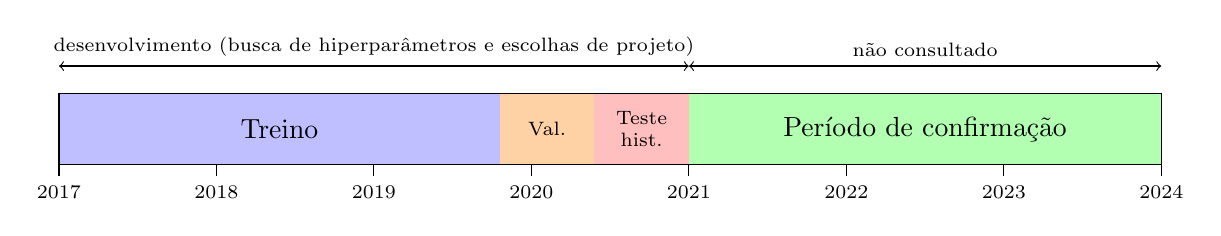
\begin{tikzpicture}[x=1cm,y=1cm]
        % escala: 1 ano = 2 cm (2017-01 -> 2024-01 = 14 cm)
        \fill[blue!25]   (0,0)     rectangle (5.60,0.9);
        \fill[orange!35] (5.60,0)  rectangle (6.80,0.9);
        \fill[red!25]    (6.80,0)  rectangle (8.00,0.9);
        \fill[green!30]  (8.00,0)  rectangle (14,0.9);
        \draw (0,0) rectangle (14,0.9);
        \node at (2.8,0.45)  {Treino};
        \node[font=\scriptsize,align=center] at (6.2,0.45) {Val.};
        \node[font=\scriptsize,align=center] at (7.4,0.45) {Teste\\hist.};
        \node at (11,0.45)   {Período de confirmação};
        \foreach \x/\y in {0/2017,2/2018,4/2019,6/2020,8/2021,10/2022,12/2023,14/2024}{
            \draw (\x,0) -- (\x,-0.15); \node[font=\scriptsize,below] at (\x,-0.15) {\y};
        }
        \draw[<->] (0,1.25) -- (8,1.25) node[midway,above,font=\scriptsize] {desenvolvimento (busca de hiperparâmetros e escolhas de projeto)};
        \draw[<->] (8,1.25) -- (14,1.25) node[midway,above,font=\scriptsize] {não consultado};
    \end{tikzpicture}%
    }
    \caption{Linha do tempo da divisão cronológica. A escala é aproximada. Val.: validação; Teste hist.: teste histórico.}
    \label{fig:split_datas_sapo}
\end{figure}

\section{Pré-processamento}
\label{sec:preprocessamento}

O pré-processamento foi desenhado para evitar vazamento temporal (Seção~\ref{sec:dados_faltantes_imputacao}). Os valores ausentes são preenchidos por interpolação linear no tempo apenas dentro do trecho de treino. Depois do fim do treino, não se usam medições futuras: a transformação apenas repete o último valor disponível até que uma nova medição apareça. Para cada variável preenchida, mantém-se um indicador de ausência, uma variável que vale 1 nos instantes em que o valor original estava faltando. O conjunto de dados é uma função determinística do arquivo original e da data de corte do treino, o que permite recriá-lo com qualquer corte.

Essa propriedade é essencial para a busca de hiperparâmetros. Em etapas exploratórias anteriores, o arquivo já preenchido era reutilizado antes de formar as partições da validação, de modo que a interpolação podia consultar valores posteriores ao corte de uma partição. Na comparação final, cada partição da validação por janela expansiva recria o conjunto a partir do arquivo original cortado no fim do seu próprio treino, com o preenchimento ajustado até esse ponto. Testes automatizados verificam que alterar valores originais posteriores ao corte não muda nenhuma linha anterior a ele.

A imputação tem duas consequências. Primeiro, em lacunas longas posteriores ao corte, a entrada do modelo fica constante (por exemplo, na lacuna de 48 dias da validação); isso reproduz o que ocorreria em operação, mas significa que parte das janelas contém valores repetidos, e sua fração é informada na Tabela~\ref{tab:splits}. Segundo, a interpolação linear dentro do treino usa valores posteriores do próprio treino, enquanto na inferência só é possível repetir o último valor; os indicadores de ausência atenuam essa diferença, mas não a eliminam.

A normalização coloca cada variável em escala comparável, subtraindo a média e dividindo pelo desvio-padrão, conforme a Equação~\ref{eq:normalizacao}.

\begin{equation}
    \tilde{x}_{t}=\frac{x_{t}-\mu_{\text{treino}}}{\sigma_{\text{treino}}}
    \label{eq:normalizacao}
\end{equation}

Na Equação~\ref{eq:normalizacao}, \(\mu_{\text{treino}}\) e \(\sigma_{\text{treino}}\) são a média e o desvio-padrão da variável, calculados somente com o bloco de treino e aplicados igualmente aos blocos de validação e de teste.

\section{Variáveis}
\label{sec:variaveis}

O conjunto de variáveis foi mantido enxuto, pois só o PM2,5, o PM10 e as partículas totais em suspensão têm medições (Seção~\ref{sec:dados}). O codificador (ou a entrada, nos modelos sem codificador) recebe o PM2,5, o PM10, seus indicadores de ausência e atributos de calendário. Os modelos que aceitam entradas para o horizonte futuro recebem apenas variáveis cujo valor pode ser determinado no instante de emissão: termos periódicos e duas variáveis derivadas do PM10. A Tabela~\ref{tab:variaveis_contrato} resume os grupos.

\begin{table}[htb]
    \centering
    \caption{Variáveis utilizadas pelos modelos.}
    \label{tab:variaveis_contrato}
    \resizebox{\textwidth}{!}{%
    \begin{tabular}{lll}
        \toprule
        \textbf{Grupo} & \textbf{Variáveis} & \textbf{Uso} \\
        \midrule
        Alvo e histórico & PM2,5 & Entrada histórica e valor a prever \\
        Poluente auxiliar & PM10 & Entrada histórica \\
        Ausência & Indicadores de ausência do PM2,5 e do PM10 & Informar quais valores foram preenchidos \\
        Calendário & Hora do dia, dia da semana e mês & Ciclos discretos \\
        Termos periódicos & Seno e cosseno com períodos de 6, 12, 24, 168 e 8760 horas & Ciclos contínuos \\
        PM10 do dia anterior & PM10 na mesma hora, 24 horas antes & Informação sobre o PM10 conhecida no instante de emissão \\
        Tendência do PM10 & PM10 24 horas antes menos PM10 27 horas antes & Direção recente do PM10, também conhecida no instante de emissão \\
        \bottomrule
    \end{tabular}%
    }
\end{table}

As duas variáveis derivadas do PM10 usam valores defasados de 24 e 27 horas em relação ao instante previsto. Como a previsão é emitida em \(t\) e o instante previsto está no máximo em \(t+24\), essas defasagens são sempre anteriores a \(t\), e não pressupõem conhecer o PM10 futuro.

Distinguem-se dois papéis das variáveis. As \emph{covariáveis do passado} são conhecidas apenas até o instante de emissão \(t\): PM2,5, PM10, seus indicadores, o calendário e os termos periódicos das 48 horas anteriores. As \emph{covariáveis futuras conhecidas} têm valor determinável em \(t\) para cada hora do horizonte: os 20 termos periódicos (seno e cosseno) e as duas variáveis derivadas do PM10. Nenhum valor observado depois de \(t\) entra em nenhum modelo. O conjunto de variáveis, a janela de 48 horas e a lista de covariáveis futuras são idênticos para todos os modelos; o que difere é a forma de consumi-los. A LSTM e o Seq2Seq recebem a janela como sequência, e as covariáveis futuras separadamente. O XGBoost e a regressão Ridge recebem a janela em uma única linha (\(48\times 30\) valores, contando um identificador constante da estação) concatenada às 23 covariáveis futuras de cada uma das 24 horas, o que totaliza 1.992 atributos. Um teste automatizado verifica que a lista de covariáveis futuras é a mesma em todos os modelos.

\section{Modelos}
\label{sec:modelos}

Foram comparadas cinco redes neurais e um modelo baseado em árvores, além de referências simples e de uma regressão linear (Tabela~\ref{tab:modelos_metodologia}). Nos nomes, ``padrão'' e ``adaptado'' referem-se às duas versões do Seq2Seq com atenção descritas adiante.

\begin{table}[htb]
    \centering
    \caption{Modelos e referências avaliados.}
    \label{tab:modelos_metodologia}
    \resizebox{\textwidth}{!}{%
    \begin{tabular}{lll}
        \toprule
        \textbf{Modelo} & \textbf{Descrição} & \textbf{Papel na comparação} \\
        \midrule
        LSTM recursiva & Prevê uma hora por vez e reinsere a previsão como entrada & Estratégia recursiva \\
        LSTM direta & Produz as 24 horas de uma vez a partir do estado final da janela & Estratégia direta \\
        Seq2Seq básico & Codificador e decodificador recorrentes, sem atenção & Codificador-decodificador mínimo \\
        Seq2Seq atenção padrão & Codificador-decodificador com atenção aditiva sobre as 48 posições & Atenção como proposta na literatura \\
        Seq2Seq atenção adaptado & Seq2Seq com atenção com quatro modificações (descritas adiante) & Variante desenhada para esta série \\
        XGBoost por horizonte & Um modelo de árvores impulsionadas para cada uma das 24 horas & Modelo baseado em árvores \\
        Previsores ingênuos & Repetição de valores passados (definidos adiante) & Piso de desempenho \\
        Regressão Ridge & Regressão linear regularizada, um modelo por horizonte & Referência linear \\
        \bottomrule
    \end{tabular}%
    }
\end{table}

\subsection{Redes Recorrentes e Seq2Seq}

A \textbf{LSTM direta} lê a janela de 48 horas e agrega os estados da sequência (pelo último estado, pela média ou por atenção, o que é escolhido na busca de hiperparâmetros) em um vetor, do qual uma camada final produz as 24 previsões de uma vez, junto com as covariáveis futuras conhecidas. A \textbf{LSTM recursiva} prevê apenas uma hora à frente e realimenta a previsão para obter as horas seguintes, mantendo as covariáveis futuras conhecidas de cada hora. O \textbf{Seq2Seq básico} usa um codificador LSTM e um decodificador LSTM autorregressivo sem atenção; durante o treinamento, o decodificador recebe o valor real anterior (\textit{teacher forcing}, Seção~\ref{sec:teacher_forcing}).

O \textbf{Seq2Seq com atenção padrão} usa o codificador LSTM, o decodificador LSTM e a atenção aditiva de \citeonline{bahdanau2014neural} (Equação~\ref{eq:atencao_aditiva}) sobre as 48 posições da janela, com a entrada do passo anterior fornecida ao decodificador (\textit{input feeding}, \citeonline{luong2015effective}). Em ambas as versões com atenção, o decodificador é \emph{semidireto}: em vez da previsão ou do valor real do passo anterior, ele recebe em todos os passos o último valor observado em \(t\), as covariáveis futuras conhecidas do horizonte e o contexto de atenção. Assim, cada horizonte depende apenas dessas entradas e do estado do codificador, e o modelo se comporta como um preditor direto, sem realimentação de previsões, o que elimina o acúmulo de erros e torna o \textit{teacher forcing} irrelevante para elas. O codificador também inclui uma seleção contextual das variáveis de entrada, inspirada na atenção de entrada do modelo DA-RNN (\textit{Dual-stage Attention-based Recurrent Neural Network}) \cite{qin2017darnn}, e uma camada linear que liga diretamente as entradas do passo à saída \cite{cheng2016wide}.

O \textbf{Seq2Seq com atenção adaptado} altera quatro pontos do padrão. Primeiro, o estado do decodificador é reiniciado a cada horizonte, de modo que cada hora é prevista de forma independente das demais. Segundo, não usa \textit{input feeding}. Terceiro, a consulta de atenção é condicionada ao número do horizonte e às covariáveis futuras. Quarto, a atenção é calculada sobre seis faixas de defasagem, e não sobre as 48 posições: a última hora, as últimas 6 horas, as últimas 24 horas, o mesmo horário do dia anterior, o mesmo horário de dois dias antes e o restante da janela, cada faixa resumida pela média dos estados do codificador naquelas posições. Essas quatro alterações são decisões de projeto, motivadas pela estrutura diária da série, e não métodos estabelecidos na literatura; por isso são avaliadas uma a uma (Seção~\ref{sec:fatores}).

\subsection{Previsores de Referência}
\label{sec:referencias_comparacao}

Sem referências simples, um erro isolado não indica se o modelo agrega valor \cite{makridakis2018statistical}. Foram usados cinco previsores ingênuos clássicos \cite{hyndman2021forecasting}. Seja \(y(t)\) o valor mais recente da série no instante de emissão \(t\) e \(\hat{y}(t+h)\) a previsão para o horizonte \(h=1,\ldots,24\):

\begin{itemize}
    \item \textbf{Persistência:} \(\hat{y}(t+h)=y(t)\), isto é, repete o último valor;
    \item \textbf{Sazonal de 24 horas:} \(\hat{y}(t+h)=y(t+h-24)\), o valor da mesma hora no dia anterior;
    \item \textbf{Sazonal de 48 horas:} \(\hat{y}(t+h)=y(t+h-48)\);
    \item \textbf{Média móvel de 6 horas:} \(\hat{y}(t+h)=\frac{1}{6}\sum_{k=0}^{5} y(t-k)\);
    \item \textbf{Média móvel de 24 horas:} \(\hat{y}(t+h)=\frac{1}{24}\sum_{k=0}^{23} y(t-k)\).
\end{itemize}

Os valores \(y(\cdot)\) vêm da série já preenchida, como nos modelos. Além disso, a regressão Ridge \cite{hoerl1970ridge}, uma regressão linear com penalização dos coeficientes, usa o mesmo vetor de 1.992 atributos do XGBoost, padronizado com as estatísticas do treino, com o coeficiente de penalização escolhido na validação entre \(\{0{,}1;\,1;\,10;\,10^2;\,10^3;\,10^4\}\). Ela mede quanto do desempenho é explicado por uma relação linear nesses atributos. A habilidade (Seção~\ref{sec:metricas_avaliacao}) usa a média móvel de 24 horas como referência, por ser o melhor previsor ingênuo em etapas exploratórias anteriores.

\subsection{XGBoost e Regressão Ridge por Horizonte}

O XGBoost e a regressão Ridge seguem a estratégia direta \cite{taieb2012review}: um modelo para cada horizonte, todos com os mesmos hiperparâmetros. Cada modelo é treinado com todas as janelas cujo alvo, \emph{naquele horizonte}, foi medido; as linhas restantes recebem peso zero. Essa é a mesma regra das redes, em que apenas os pontos sem medição ficam fora da perda. Uma versão anterior treinava um único modelo com as 24 saídas e exigia as 24 medidas na mesma janela, o que descartava cerca de 70\% das janelas de treino e esgotava a memória de uma placa de vídeo de 8~GB; ela foi abandonada por criar uma desvantagem de dados para o XGBoost. O objetivo de treinamento do XGBoost é o erro absoluto, consistente com o MAE \cite{gneiting2011making}.

\subsection{Fatores Estudados}
\label{sec:fatores}

Para que as diferenças entre modelos possam ser atribuídas à sua causa, quatro fatores que variavam juntos em etapas anteriores foram separados. Cada um é alterado sozinho em relação a um caso base.

\begin{enumerate}
    \item \textbf{Arquitetura}, comparada com a perda de Huber e sem aprendizado residual em todas as redes (comparação principal).
    \item \textbf{Função de perda:} perda de Huber contra uma perda absoluta ponderada, aplicada a todas as arquiteturas. A perda ponderada multiplica o erro absoluto por pesos maiores quando o valor observado excede 15 e 35~\(\mu\)g/m\(^3\), e por um fator adicional quando a previsão fica abaixo de um valor alto (Equação~\ref{eq:perda_ponderada}). Os pesos são uma decisão de projeto, fixos e motivados pelo aprendizado sensível ao custo \cite{elkan2001foundations} e pela ideia de penalizar de forma assimétrica os erros de subestimação, como nas perdas quantílicas \cite{koenker1978regression}.
    \item \textbf{Aprendizado residual:} a rede prevê a correção sobre uma previsão de base, \(\hat{y}_{t+k}=b_{t+k}+g_{\theta}(\cdot)\), em que \(b_{t+k}\) é a média entre o último valor observado e os valores de 24 e 48 horas antes do instante previsto, uma composição de previsores ingênuos. Está disponível para a LSTM direta e para o Seq2Seq adaptado.
    \item \textbf{Perda auxiliar de evento:} uma saída adicional do Seq2Seq adaptado prevê, durante o treinamento, se haverá concentração acima de 25 e de 35~\(\mu\)g/m\(^3\), segundo a lógica de aprendizado com várias tarefas \cite{caruana1997multitask}.
\end{enumerate}

\begin{equation}
    \mathcal{J}_{w}
    =
    \frac{\sum_{(i,k)\in\mathcal{O}}w_{i,k}\,|y_{i,k}-\hat{y}_{i,k}|}
    {\sum_{(i,k)\in\mathcal{O}}w_{i,k}}
    \label{eq:perda_ponderada}
\end{equation}

Na Equação~\ref{eq:perda_ponderada}, \(\mathcal{O}\) é o conjunto de pares (exemplo \(i\), horizonte \(k\)) cujo valor foi efetivamente medido, \(y_{i,k}\) é o valor observado, \(\hat{y}_{i,k}\) é a previsão e \(w_{i,k}\) é o peso definido acima. Esta é uma perda absoluta ponderada sobre as previsões, e não uma regularização dos parâmetros.

Além disso, cada uma das quatro alterações do Seq2Seq adaptado é removida individualmente, mantendo os hiperparâmetros do modelo completo, para medir sua contribuição. E as variáveis do PM10 são removidas em dois cenários: mantendo o PM10 apenas no histórico (sem as duas variáveis derivadas para o futuro) e removendo o PM10 por completo, para a LSTM direta e para o XGBoost, cada cenário com sua própria busca de hiperparâmetros.

\subsection{O Que É Igual e O Que Muda Entre os Modelos}

A Tabela~\ref{tab:protocolo_igual} lista o que é idêntico para todos os modelos e a Tabela~\ref{tab:protocolo_casos} lista, caso a caso, o que muda. Três diferenças não podem ser eliminadas: (i) o XGBoost não tem épocas nem agenda de taxa de aprendizado, usa a parada antecipada própria e não aceita a perda ponderada; (ii) a LSTM recursiva realimenta a própria previsão e, por isso, não tem versão com aprendizado residual; (iii) os casos que alteram apenas a perda, o aprendizado residual ou o desenho reaproveitam os hiperparâmetros encontrados para o caso de Huber da mesma arquitetura, o que isola o efeito do fator, ao custo de possivelmente subestimar cada variante. O efeito desse reaproveitamento é verificado refazendo a busca para a perda ponderada em duas arquiteturas (Seção~\ref{sec:sensibilidades}).

\inputtabela{protocolo_igual}

\inputtabela{protocolo_casos}

Transformers para séries temporais, como o \textit{Temporal Fusion Transformer}, o Informer, o Autoformer e o PatchTST \cite{lim2021tft,zhou2021informer,wu2021autoformer,nie2023patchtst}, não foram incluídos: uma comparação justa exigiria outro espaço de hiperparâmetros, um orçamento de busca equivalente e várias sementes. Além disso, a literatura não indica que eles superem automaticamente os demais modelos \cite{zeng2023transformers}. O recorte deste estudo é comparar redes recorrentes, modelos baseados em árvores e referências simples sob o mesmo tratamento dos dados.

\section{Treinamento e Busca de Hiperparâmetros}
\label{sec:treinamento_hpo}

Todos os modelos passam pelo mesmo procedimento (Tabela~\ref{tab:protocolo_igual}). Os hiperparâmetros de cada arquitetura são escolhidos por validação por janela expansiva com três partições (Seção~\ref{sec:validacao_temporal}), dentro dos blocos de treino e validação e sem acesso ao teste histórico nem ao período de confirmação. Cada partição recria a série preenchida a partir do arquivo original cortado no seu fim, e o critério de escolha é o MAE médio das partições, calculado apenas em alvos medidos. O orçamento é o mesmo para todas as famílias: 24 tentativas por arquitetura, com até 18 épocas por tentativa nas redes e a parada antecipada própria no XGBoost. Durante a busca, as janelas de treino avançam de 4 em 4 horas por custo computacional; o treino final avança de 2 em 2 horas e a avaliação, de 1 em 1 hora, para todos os modelos.

Nas redes, o estudo do Optuna usa o amostrador TPE com semente fixa e a poda \textit{Hyperband}, que exige um mínimo de 4 épocas antes de podar uma tentativa (as 3 primeiras épocas são de aquecimento da taxa de aprendizado, em que o erro ainda não é representativo), com no máximo 18 épocas e fator de redução 3 \cite{akiba2019optuna,li2018hyperband}. Como o recurso é a época, só a primeira partição informa valores intermediários e pode podar a tentativa; a métrica da tentativa continua sendo a média das partições. No XGBoost, a busca minimiza o MAE médio das partições com TPE e poda pela mediana \cite{optunaDocsMedian2026,chen2016xgboost}. Os 24 modelos por horizonte do XGBoost são treinados na placa de vídeo, sem retorno automático ao processador: uma configuração que esgotasse a memória seria podada e contada, mas isso não ocorreu, e o pico medido foi de cerca de 1,4~GB entre os 8~GB disponíveis. As Tabelas~\ref{tab:hpo_espaco_busca} e \ref{tab:hpo_melhores} apresentam, respectivamente, o espaço de busca e a configuração escolhida.

O treino final usa o AdamW \cite{loshchilov2019decoupled}. A taxa de aprendizado tem três épocas de aquecimento linear, de \(10^{-5}\eta_{\max}\) a \(\eta_{\max}\), seguidas de decaimento cosseno até \(0{,}01\,\eta_{\max}\) no fim das 40 épocas \cite{goyal2017accurate,loshchilov2017sgdr}. A validação, ao fim de cada época, mede o MAE e serve à parada antecipada (paciência de 8 épocas) e à escolha do melhor ponto do treinamento. Cada modelo é treinado com várias \emph{sementes}, isto é, várias inicializações aleatórias dos pesos: quatro (42, 7, 21 e 123) na comparação principal e as três primeiras nos demais grupos, que respondem a perguntas sobre o efeito de um fator e não à classificação entre modelos. A média das previsões das sementes forma um \emph{ensemble}, reportado à parte \cite{lakshminarayanan2017simple}.

\begin{table}[htb]
    \centering
    \caption{Espaço de busca de hiperparâmetros.}
    \label{tab:hpo_espaco_busca}
    \small
    \renewcommand{\arraystretch}{1.08}
    \begin{tabular}{>{\raggedright\arraybackslash}p{0.22\textwidth}>{\raggedright\arraybackslash}p{0.23\textwidth}>{\raggedright\arraybackslash}p{0.45\textwidth}}
        \toprule
        \textbf{Grupo} & \textbf{Hiperparâmetro} & \textbf{Valores avaliados} \\
        \midrule
        Redes neurais & Taxa de aprendizado & 0,0004; 0,0008; 0,0012; 0,0018; 0,0025; 0,0035; 0,005; 0,007 \\
        Redes neurais & Decaimento de pesos & 0; \(10^{-6}\); \(5\times10^{-6}\); \(10^{-5}\); \(5\times10^{-5}\); \(10^{-4}\) \\
        Redes neurais & \textit{Dropout} e camadas & \textit{dropout} de 0,05 a 0,30 (passo 0,05); 1, 2 ou 3 camadas \\
        Redes neurais (Huber) & \(\delta\) da perda de Huber & 0,5; 1,0; 1,5; 2,0 \\
        LSTM direta & Arquitetura & unidades ocultas de 64 a 320; agregação por último estado, média ou atenção \\
        LSTM recursiva & Arquitetura & unidades ocultas de 64 a 320 \\
        Seq2Seq básico & Arquitetura & unidades ocultas de 64 a 256 \\
        Seq2Seq com atenção & Arquitetura & codificador com 64 a 160 unidades; decodificador com 64 a 192; atenção com 64 a 128; representação do horizonte com 8, 16, 24 ou 32 dimensões \\
        XGBoost & Árvores e profundidade & 160, 240, 320 ou 480 árvores; profundidade de 2 a 7; \texttt{max\_bin} 64, 128 ou 256 \\
        XGBoost & Regularização e amostragem & taxa de aprendizado entre 0,015 e 0,12 (escala logarítmica); \textit{subsample} e \textit{colsample} entre 0,60 e 1,0; \(\lambda\), \(\alpha\), \(\gamma\) e peso mínimo do filho; parada antecipada após 10, 15 ou 25 rodadas \\
        \bottomrule
    \end{tabular}
\end{table}

\inputtabela{hpo_melhores}

\section{Métricas de Avaliação}
\label{sec:metricas}

As métricas globais são as da Seção~\ref{sec:metricas_avaliacao}: MAE, RMSE, \(R^2\), MBE, WAPE e sMAPE, além do MAPE. Como o alvo é baixo e inteiro (mediana próxima de 10~\(\mu\)g/m\(^3\) e mínimo de 1), o MAPE é reportado apenas como referência; o WAPE e o sMAPE acompanham o MAE \cite{hyndman2006another}. Também se reporta o MAE nos horizontes 1 e 24, e a habilidade em relação à média móvel de 24 horas.

Para os picos, definem-se o MAE, o viés e a taxa de subestimação (fração das horas em que a previsão fica abaixo do observado) restritos às horas com PM2,5 acima de 25, 35 e 50~\(\mu\)g/m\(^3\), e a razão entre os desvios-padrão da previsão e da observação, que mede o quanto a previsão é suavizada, além do percentil 99 previsto. O limiar de 35~\(\mu\)g/m\(^3\) é uma escolha de projeto, próxima ao padrão intermediário de 37~\(\mu\)g/m\(^3\) para 24 horas da Resolução CONAMA nº 491/2018 \cite{conama2018res491}, e produz eventos em número suficiente; os limiares 25 e 50 verificam a sensibilidade a essa escolha. Um \emph{evento} é uma sequência de horas consecutivas medidas com PM2,5 acima do limiar; para cada evento calculam-se o MAE, o viés, a taxa de subestimação e o erro na hora do pico. A dinâmica horária é avaliada por três medidas sobre pares de horas consecutivas: a correlação entre os níveis, a correlação entre as diferenças de uma hora para a seguinte e a fração de vezes em que a direção da mudança (subida ou descida) é acertada. Elas separam acertar o nível de acertar o momento das mudanças.

\paragraph{Tratamento dos valores preenchidos.} As métricas são calculadas somente sobre alvos efetivamente medidos, e a perda de treinamento também os ignora. Esta é uma escolha do trabalho, e não uma convenção geral da área de qualidade do ar. Ela tem precedente em previsão com dados faltantes: \citeonline{li2018dcrnn} excluem os valores ausentes do cálculo do MAE, do RMSE e do MAPE em previsão de tráfego, e \citeonline{che2018recurrent} tratam a ausência como informação de entrada, na linha dos indicadores de ausência usados aqui. A justificativa é que um alvo preenchido é uma estimativa (aqui, uma interpolação linear); avaliar contra ele mediria a aderência à interpolação, e não ao fenômeno, e favoreceria previsões suaves. Não encontramos trabalho de previsão de PM2,5 que trate explicitamente dessa escolha; por isso ela é uma decisão metodológica, acompanhada de uma análise de sensibilidade (Seção~\ref{sec:sensibilidades}) que reporta o MAE incluindo os pares preenchidos. As conclusões só são consideradas robustas a essa escolha se a ordenação dos modelos se mantiver. Uma limitação é a possível ausência informativa (falhas do instrumento concentradas em altas concentrações) \cite{littlerubin2019statistical}, que a exclusão não corrige.

\section{Inferência Estatística}
\label{sec:inferencia_estatistica}

Cada hora prevista aparece em cerca de 24 janelas sobrepostas, e os erros são autocorrelacionados; tratar os pares como independentes superestimaria a precisão (Seção~\ref{sec:comparacao_estatistica}). As diferenças entre modelos são avaliadas de três formas.

\begin{enumerate}
    \item \textbf{Bootstrap em blocos, pareado.} Para cada instante de emissão, somam-se os erros absolutos (ou quadráticos) e a quantidade de pares medidos. Sorteiam-se blocos circulares de 168 horas consecutivas (uma semana) \cite{politis1992circular,kunsch1989jackknife}, com os mesmos blocos para os dois modelos comparados e 2.000 repetições, e obtém-se o intervalo de 95\% da diferença do MAE (ou do RMSE). Um intervalo que contém zero indica empate estatístico.
    \item \textbf{Teste de Diebold-Mariano} \cite{diebold1995comparing}, sobre a série das diferenças de perda média por instante de emissão, com variância de longo prazo de Newey-West \cite{newey1987simple} (defasagem 23, que cobre a dependência induzida pelas janelas de 24 horas) e a correção de amostra pequena de \citeonline{harvey1997testing}.
    \item \textbf{Bootstrap sobre eventos}, na comparação por evento de pico, sorteando os eventos.
\end{enumerate}

Para estimar a diferença entre famílias de modelos, e não a de uma semente em particular, as comparações usam a média das estatísticas entre as sementes de cada caso; a variabilidade entre sementes é reportada à parte. As comparações são feitas contra duas referências fixadas antes da execução: a LSTM direta com perda de Huber, por ter sido o melhor modelo em etapas exploratórias anteriores, e a média móvel de 24 horas. Todas as tabelas e testes são gerados por um programa a partir das previsões salvas, sem retreinar os modelos.

\section{Verificações de Sensibilidade}
\label{sec:sensibilidades}

Três verificações testam se as conclusões dependem de escolhas de projeto. A primeira varia a janela de entrada em 24, 48, 72 e 96 horas, com o horizonte fixo em 24 horas, para a LSTM direta e para o XGBoost; os hiperparâmetros são os do caso de 48 horas, e a comparação usa exclusivamente o MAE de \emph{validação}, de modo que o teste não participa da escolha (Seção~\ref{sec:sensibilidade_janela}). A segunda recalcula o MAE incluindo, além das medições, os pares cujo alvo foi preenchido. A terceira refaz a busca de hiperparâmetros para a perda ponderada na LSTM direta e no Seq2Seq adaptado, para medir o viés de reaproveitar os hiperparâmetros do caso de Huber.

\section{Diagnóstico da Atenção}
\label{sec:diagnostico_atencao}

Os pesos de atenção nem sempre indicam a importância de uma entrada \cite{jain2019attention,serrano2019attention,wiegreffe2019attention}. Por isso a leitura da atenção usa dois instrumentos. O primeiro são medidas dos pesos: a entropia normalizada (1 para pesos uniformes e menor quando os pesos se concentram), o peso máximo e a fração do peso total (massa) concentrada na última hora, nas últimas seis horas e nas posições do mesmo horário de um e de dois dias antes. Para pesos uniformes sobre 48 posições, cada posição recebe \(1/48\approx0{,}021\). O segundo é uma contraprova feita sem novo treinamento: os pesos aprendidos são substituídos por pesos uniformes, por pesos uniformes dentro de cada faixa de defasagem, apenas pela última hora, apenas pela posição de 24 ou de 48 horas antes, ou o contexto é zerado, e mede-se a variação do erro. Se um padrão fixo produz erro equivalente ao da atenção aprendida, a atenção aprendida não é decisiva para a previsão, independentemente do seu aspecto. \citeonline{cinar2017position} argumentam que a atenção de \citeonline{bahdanau2014neural} não atende por si só à sazonalidade de séries temporais; a variante adaptada, com faixas de defasagem alinhadas ao dia anterior, é uma resposta estrutural a essa limitação.

\section{Reprodutibilidade}
\label{sec:reprodutibilidade}

Toda a execução é orquestrada por um programa único, com o procedimento definido em arquivos de configuração e testes automatizados que verificam que o treino é idêntico entre os casos e que a construção dos dados não vaza informação posterior ao corte. Cada execução grava as sementes, os hiperparâmetros, o código de identificação dos dados, a versão do código e a indicação de árvore de código limpa. As tabelas do Capítulo~\ref{chap:resultados} são geradas por programa e incluídas diretamente no texto, sem transcrição manual. O código e os comandos de reprodução acompanham o repositório técnico do trabalho.
